%%%%%%%%%%%%%%%%%%%%%%%%%%%%%%%%%%%%%%%%%
% a0poster Portrait Poster
% LaTeX Template
% Version 1.0 (22/06/13)
%
% The a0poster class was created by:
% Gerlinde Kettl and Matthias Weiser (tex@kettl.de)
% 
% This template has been downloaded from:
% http://www.LaTeXTemplates.com
%
% License:
% CC BY-NC-SA 3.0 (http://creativecommons.org/licenses/by-nc-sa/3.0/)
%
%%%%%%%%%%%%%%%%%%%%%%%%%%%%%%%%%%%%%%%%%

%----------------------------------------------------------------------------------------
%	PACKAGES AND OTHER DOCUMENT CONFIGURATIONS
%----------------------------------------------------------------------------------------

\documentclass[a0,portrait]{a0poster}



\usepackage{multicol} % This is so we can have multiple columns of text side-by-side
\columnsep=100pt % This is the amount of white space between the columns in the poster
\columnseprule=3pt % This is the thickness of the black line between the columns in the poster

\usepackage[svgnames]{xcolor} % Specify colors by their 'svgnames', for a full list of all colors available see here: http://www.latextemplates.com/svgnames-colors

\usepackage{times} % Use the times font
%\usepackage{palatino} % Uncomment to use the Palatino font

\usepackage{graphicx} % Required for including images
\graphicspath{{figures/}} % Location of the graphics files
\usepackage{booktabs} % Top and bottom rules for table
\usepackage[font=small,labelfont=bf]{caption} % Required for specifying captions to tables and figures
\usepackage{amsfonts, amsmath, amsthm, amssymb} % For math fonts, symbols and environments
\usepackage{wrapfig} % Allows wrapping text around tables and figures
\usepackage{inconsolata}
\usepackage{listings}
\lstdefinelanguage{pseudi}{
	basicstyle=\ttfamily,
	showstringspaces=false,
	literate={:}{{{\color{RoyalBlue}:}}}1,
	keywords={for, each, in},
	ndkeywords={Map},
	sensitive=false,
	comment=[l]{//},
}
\usepackage{mathpazo} % add possibly `sc` and `osf` options
\usepackage{eulervm}

\begin{document}

%----------------------------------------------------------------------------------------
%	POSTER HEADER 
%----------------------------------------------------------------------------------------

% The header is divided into two boxes:
% The first is 75% wide and houses the title, subtitle, names, university/organization and contact information
% The second is 25% wide and houses a logo for your university/organization or a photo of you
% The widths of these boxes can be easily edited to accommodate your content as you see fit

\begin{minipage}[b]{0.75\linewidth}
\Huge \color{NavyBlue} \textbf{THoSP: an Algorithm for Nesting Property Graphs} \color{Black}\\ % Title
%\Huge\textit{An Exploration of Complexity}\\[2cm] % Subtitle
\huge \textbf{Giacomo Bergami\textsuperscript{1}, Andr\'e Petermann\textsuperscript{2}, Danilo Montesi\textsuperscript{1}}\\[0.5cm] % Author(s)
\huge Universit\`a di Bologna\textsuperscript{1}, Universit\"at Leipzig\textsuperscript{2}\\[0.4cm] % University/organization
\Large \texttt{bergamigiacomo@gmail.com}\\
\end{minipage}
%
%\begin{minipage}[b]{0.25\linewidth}
%\includegraphics[width=20cm]{logo.png}\\
%\end{minipage}

\vspace{1cm} % A bit of extra whitespace between the header and poster content

%----------------------------------------------------------------------------------------

\begin{multicols}{2} % This is how many columns your poster will be broken into, a portrait poster is generally split into 2 columns

%----------------------------------------------------------------------------------------
%	ABSTRACT
%----------------------------------------------------------------------------------------

\color{Navy} % Navy color for the abstract



%----------------------------------------------------------------------------------------
%	INTRODUCTION
%----------------------------------------------------------------------------------------

\color{SaddleBrown} % SaddleBrown color for the introduction

\section*{Abstract/Introduction}

 Despite the growing popularity of techniques related to graph summarization, a general operator for the flexible nesting of graphs is still missing.
We propose a novel nested graph data model and a powerful graph nesting operator. In contrast to existing approaches, our approach is able to summarize vertices and paths among vertex groups within a single query. Further on, our model supports partial nestings under the preservation of original graph elements as well as the full recovery of the original graph. We propose an efficient nesting algorithm (THoSP) that is able to perform vertex and path nestings in a single visit of the input graph. Results of an experimental evaluation show that THoSP outperforms equivalent implementations based on graph (Cypher, SPARQL), relational (SQL) and document oriented (ArangoDB) databases.

%----------------------------------------------------------------------------------------
%	OBJECTIVES
%----------------------------------------------------------------------------------------

\color{DarkSlateGray} % DarkSlateGray color for the rest of the content

\section*{Goal and Motivation.}

\begin{center}\vspace{1cm}
	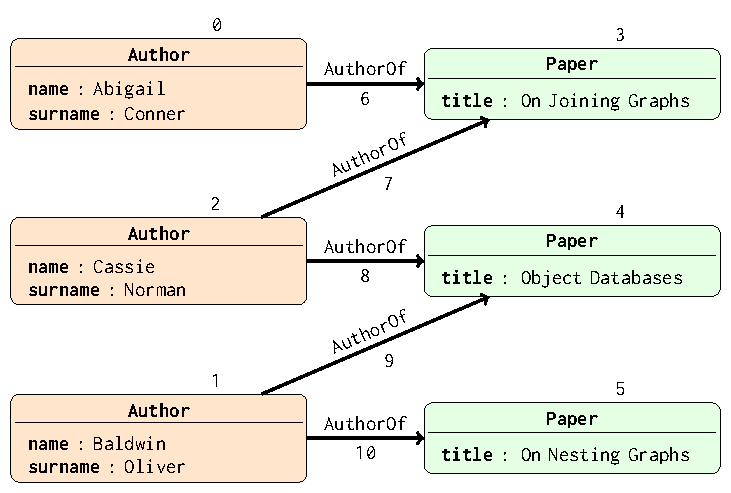
\includegraphics[width=.7\linewidth]{figures/06nesting/04bibliography.pdf}
	\captionof{figure}{\color{Green} This paper analyses one specific problem, that is perform ``graph projections'' over bibliography networks.}
\end{center}\vspace{1cm}

\begin{center}\vspace{1cm}
	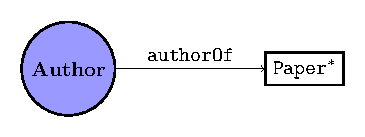
\includegraphics[width=.35\linewidth]{figures/06nesting/00_vertex_pattern.pdf}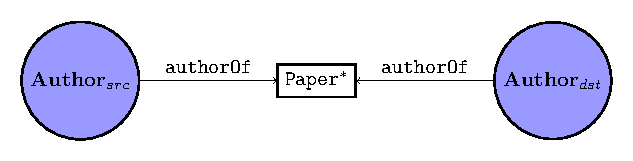
\includegraphics[width=.45\linewidth]{figures/06nesting/00_path_pattern.pdf}
	\captionof{figure}{\color{Green} This paper addressed the problem of nesting graphs by using two distinct vertex and edge patterns. The pattern contains relevant pieces of information for both matching the input graph and providing the nesting content.}
\end{center}\vspace{1cm}

\section*{Nested Graph Data Model. Features.}

\begin{center}\vspace{1cm}
	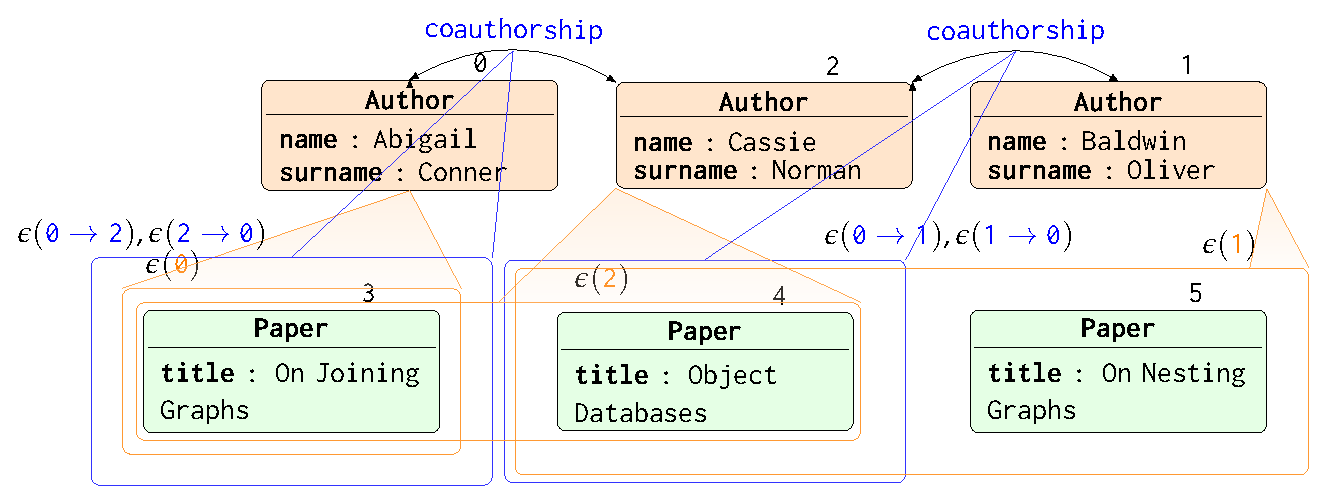
\includegraphics[width=\linewidth]{figures/06nesting/042nested.pdf}
	\captionof{figure}{\color{Green} Desired Query Result}
\end{center}\vspace{1cm}

\begin{enumerate}
\item Nested graphs is an extension of the property graph data model.
\item Each vertex and each edge may represent an (eventually empty) graph.
\item Recursive inclusion must not be allowed (containment can resembled to part-of or is-a relations \cite{Tesi}).
\end{enumerate}

%----------------------------------------------------------------------------------------
%	MATERIALS AND METHODS
%----------------------------------------------------------------------------------------

\section*{Methods and Data Sources}

This paper extends the previous property graph data model presented in \cite{BergamiMM17}, where property graphs were represented as adjacency lists. To better evaluate the contribution of the loading/indexing and the query evaluation plan, no ancillary data is associated with both authors and papers. We perform evaluations on both synthetic and real-world bibliographic data.

%------------------------------------------------
\bibliographystyle{plain} % Plain referencing style
\bibliography{sample} % Use the example bibliography file sample.bib

\subsection*{THoSP Algorithm for Two-Hop separated patterns}
\begin{lstlisting}[mathescape=true,language=pseudi]
nest(Cont, patt, u, S):
for each s in S s.t. patt.doSerialize(s):
     Cont.write(<u,s>)

Input: G, gV, gE 
Cont $\leftarrow$ $\emptyset$ 
NestedGraph $\leftarrow$ $\emptyset$ 

a $\leftarrow$ V $\cap$ E \ ($\gamma_V$ $\cup$ $\gamma_E^{src}$ $\cup$ $\gamma_E^{dst}$);
for each v:vertex in G s.t. a(v):
  for each V(u $\rightarrow^{e}$ v):
    $\textbf{u}$ := dtl(u)$_c$ ; nest(Cont, V, $\textbf{u}$, {u,e,v})
    NGraph(V) $\leftarrow$ NGraph(V) $\cup${$\textbf{u}$}
    for each V(w $\rightarrow^{e'}$ v) s.t. E(u $\rightarrow^{e}$ v${}^{e'}\leftarrow$w)
      $\textbf{w}$ := dtl(w)$_c$ ;
      $\textbf{e'}$ := dtl(u,w)$_c$; 
      nest(Cont, E, $\textbf{e'}$, {u,e,v,e',w})
      NGraph(E) $\leftarrow$ NGraph(E) $\cup${$\textbf{u} \rightarrow^{\textbf{e'}} \textbf{w}$}
	\end{lstlisting}

%----------------------------------------------------------------------------------------
%	RESULTS 
%----------------------------------------------------------------------------------------

\section*{Results}

Preliminar valuation over a synthetic dataset generated with GMark.
%
\begin{center}
\begin{tabular}{@{}c|rrrr|r@{}}
	\toprule
	\multicolumn{1}{c}{\textbf{Operand}} & \multicolumn{5}{|c}{\textbf{Operand Loading and Indexing Time (C/C++)} (ms)}  \\
	$|V|$  & {PostgreSQL} & {Virtuoso} & {ArangoDB}  &  {Neo4J (Java)} & {\textbf{Nested Graphs}}  \\
	\midrule
	$10$   & 8.00$\cdot 10^0$ & 3.67$\cdot 10^0$ & 4.30$\cdot 10^1$ & 3.95$\cdot 10^3$  & \textbf{1.30}$\cdot 10^{-1}$\\
	$10^2$  & 1.80$\cdot 10^1$ & 6.86$\cdot 10^0$ & 2.67$\cdot 10^2$ &  4.12$\cdot 10^3$ & \textbf{3.30}$\cdot 10^{-1}$\\
	$10^3$  & 4.50$\cdot 10^1$ & 2.35$\cdot 10^1$ & 1.28$\cdot 10^3$ & 5.25$\cdot 10^3$ & \textbf{3.51}$\cdot 10^0$\\
	$10^4$   & 2.25$\cdot 10^2$ & 3.71$\cdot 10^2$ & 1.15$\cdot 10^4$ &  1.12$\cdot 10^4$ & \textbf{3.18}$\cdot 10^1$\\
	$10^5$   & 1.87$\cdot 10^3$ & 3.51$\cdot 10^3$ & 1.35$\cdot 10^5$ &  1.19$\cdot 10^6$ & \textbf{3.37}$\cdot 10^2$ \\
	$10^6$  & 1.91$\cdot 10^4$ & 3.46$\cdot 10^4$ & 1.36$\cdot 10^6$ & $>$1H & \textbf{3.69}$\cdot 10^3$\\
	$10^7$   & 1.84$\cdot 10^5$ & 3.64$\cdot 10^5$ & $>$1H & $>$1H & \textbf{4.40}$\cdot 10^4$\\
	$10^8$  & 1.98$\cdot 10^6$ & $>$1H & $>$1H & $>$1H & \textbf{5.18}$\cdot 10^5$\\
	\bottomrule
\end{tabular}
\begin{tabular}{@{}cr|rrrr|r@{}}
	\toprule
	\multicolumn{2}{c}{\textbf{Operands Size}} & \multicolumn{5}{|c}{\textbf{\textsc{Two HOp Separated Pattern} Time (C/C++)} (ms)}  \\
	$|V|$  & \#Subgraph  &  {SQL+JSON} & SPARQL & AQL  &  Cypher &{\textbf{THoSP}}  \\
	\midrule
	$10$ & $3$  & 2.10$\cdot 10^0$ &  1.10$\cdot 10^1$ & 3.89$\cdot 10^0$  & 6.81$\cdot 10^2$  & \textbf{1.10}$\cdot 10^{-1}$\\
	$10^2$ & $58$  & 9.68$\cdot 10^0$ &  6.30$\cdot 10^1$ & 1.23$\cdot 10^1$  &  1.94$\cdot 10^3$ & \textbf{1.40}$\cdot 10^{-1}$\\
	$10^3$ & $968$  & 1.80$\cdot 10^1$ & 6.30$\cdot 10^1$ & 1.50$\cdot 10^1$ & $>$1H & \textbf{4.60}$\cdot 10^{-1}$\\
	$10^4$ & $8,683$  & 6.92$\cdot 10^1$ & 3.64$\cdot 10^2$ & 4.67$\cdot 10^1$ &  $>$1H & \textbf{4.07}$\cdot 10^0$\\
	$10^5$ & $88,885$  & 2.94$\cdot 10^2$ & 4.15$\cdot 10^3$ & 5.09$\cdot 10^2$ &  $>$1H & \textbf{4.38}$\cdot 10^1$ \\
	$10^6$ & $902,020$  & 2.61$\cdot 10^3$ & 5.03$\cdot 10^4$ & 7.21$\cdot 10^3$ & $>$1H & \textbf{5.63}$\cdot 10^2$\\
	$10^7$ & $8,991,417$  & 2.57$\cdot 10^4$ & 6.72$\cdot 10^5$ & 9.22$\cdot 10^5$ & $>$1H & \textbf{8.20}$\cdot 10^3$\\
	$10^8$ & $89,146,891$  & 3.96$\cdot 10^5$ & $>$1H & $>$1H & $>$1H & \textbf{9.18}$\cdot 10^4$\\
	\bottomrule
\end{tabular}
\end{center}
\medskip

Evaluation performed over an example of real world data, Microsoft Academic Graph. Please note the competitors experience some Out-Of-Memory errors before the $1H=3.6\cdot 10^6$ timeout.

\begin{center}

\begin{tabular}{@{}c|rrrr|r@{}}
	\toprule
	\multicolumn{1}{c}{\textbf{Operand}} & \multicolumn{5}{|c}{\textbf{Operand Loading and Indexing Time (C/C++)} (ms)}  \\
	$|V|$  & {PostgreSQL} & {Virtuoso} & {ArangoDB}  &  {Neo4J (Java)} & {\textbf{Nested Graphs}}  \\
	\midrule
	$10$   & 2.59$\cdot 10^1$   & 1.21$\cdot 10^1$  & 2.43$\cdot 10^2$ &  2.93$\cdot 10^3$ & \textbf{3.49}$\cdot 10^{-1}$\\
	$10^2$  & 2.80$\cdot 10^1$  & 1.22$\cdot 10^1$  & 3.91$\cdot 10^2$ & 3.10$\cdot 10^3$  & \textbf{8.87}$\cdot 10^{-1}$\\
	$10^3$  & 2.96$\cdot 10^1$  & 7.86$\cdot 10^1$  & 2.67$\cdot 10^3$ & 4.65$\cdot 10^3$ & \textbf{6.53}$\cdot 10^0$\\
	$10^4$   & \textbf{4.00}$\cdot 10^1$ & 7.43$\cdot 10^2$  & 2.34$\cdot 10^4$ & 4.23$\cdot 10^4$ & 6.90$\cdot 10^1$\\
	$10^5$   & 3.44$\cdot 10^3$ & 2.11$\cdot 10^4$  & 6.08$\cdot 10^5$ & $>$1H & \textbf{1.58}$\cdot 10^3$ \\
	$10^6$  & 1.35$\cdot 10^4$  & 1.38$\cdot 10^5$  & $>$1H & $>$1H & \textbf{1.18}$\cdot 10^4$\\
	$10^7$   & \textbf{4.77}$\cdot 10^4$ &              $>$1H  & $>$1H & $>$1H & 1.05$\cdot 10^5$\\
	%$10^8$  & -- & $>$1H & $>$1H & $>$1H & 1.08$\cdot 10^6$\\
	\bottomrule
\end{tabular}

\begin{tabular}{@{}cr|rrrr|r@{}}
	\toprule
	\multicolumn{2}{c}{\textbf{Operands Size}} & \multicolumn{5}{|c}{\textbf{\textsc{Two HOp Separated Pattern} Time (C/C++)} (ms)}  \\
	$|V|$  & \#Subgraph  &  {SQL+JSON} & SPARQL & AQL  &  Cypher &{\textbf{THoSP}}  \\
	\midrule
	$10$ & 19  & 1.69$\cdot 10^0$   &  3.4$\cdot 10^1$  & 6.57$\cdot 10^{-1}$  & 2.38$\cdot 10^3$    & \textbf{2.82}$\cdot 10^{-1}$\\
	$10^2$ & 255 & 1.75$\cdot 10^0$  & 3.22$\cdot 10^2$ & 2.51$\cdot 10^0$  & 1.01$\cdot 10^4$    & \textbf{3.46}$\cdot 10^{-1}$\\
	$10^3$ & 23,119  & 4.71$\cdot 10^1$ &  1.22$\cdot 10^3$ & 8.18$\cdot 10^1$  & $>$1H & \textbf{1.39}$\cdot 10^{1}$\\
	$10^4$ & 5,411,205  & 1.53$\cdot 10^4$ &  2.77$\cdot 10^5$ & 2.08$\cdot 10^4$  & $>$1H & \textbf{2.58}$\cdot 10^3$\\
	$10^5$ & 97,079,329  & 1.20$\cdot 10^6$ & $>$1H & {\color{red}OOM$^1$}  & $>$1H & \textbf{1.97}$\cdot 10^5$ \\
	$10^6$ & 241,448,529  & $>$1H &           $>$1H & {\color{red}OOM$^1$}  & $>$1H    & \textbf{6.22}$\cdot 10^5$\\
	$10^7$ & 361,759,509  & {\color{red}OOM$^2$} &      $>$1H & {\color{red}OOM$^1$}  & $>$1H      & \textbf{7.74}$\cdot 10^5$\\
	%$10^8$ & --  & -- & $>$1H & $>$1H & $>$1H & --\\
	\bottomrule
\end{tabular}
\end{center}
%----------------------------------------------------------------------------------------
%	CONCLUSIONS
%----------------------------------------------------------------------------------------

\color{SaddleBrown} % SaddleBrown color for the conclusions to make them stand out

\section*{Conclusions}

\begin{itemize}
\item This paper proposed for the first time an algorithm (THoSP) which adds the structural aggregation to an input graph.
\item Both the logical data model and the query result separate the graph representation from
the actual containment information.
\item Containment indices quicken summarisation tasks by avoiding reordering costs.
\item Given two graph patterns, it is possible to detect the commonly shared subpattern to reduce the graph visiting costs. This solution provides an optimal graph visiting cost.
\end{itemize}


\color{DarkSlateGray} % Set the color back to DarkSlateGray for the rest of the content

%----------------------------------------------------------------------------------------
%	FORTHCOMING RESEARCH
%----------------------------------------------------------------------------------------

\section*{Forthcoming Research}

\begin{itemize}
	\item Extend the class of optimizable graph nesting patterns for data integration scenarios (see GROQ in \cite{Tesi}), implement the algorithm and implement the benchmarks.
	\item A more general data model may provide a more elegant definition of the proposed graph nesting operator.
\end{itemize}

 %----------------------------------------------------------------------------------------
%	REFERENCES
%----------------------------------------------------------------------------------------


%----------------------------------------------------------------------------------------
%	ACKNOWLEDGEMENTS
%----------------------------------------------------------------------------------------

%\section*{Acknowledgements}
%Etiam fermentum, arcu ut gravida fringilla, dolor arcu laoreet justo, ut imperdiet urna arcu a arcu. Donec nec ante a dui tempus consectetur. Cras nisi turpis, dapibus sit amet mattis sed, laoreet.

%----------------------------------------------------------------------------------------

\end{multicols}
\end{document}
